\PassOptionsToPackage{unicode=true}{hyperref} % options for packages loaded elsewhere
\PassOptionsToPackage{hyphens}{url}
%
\documentclass[11pt,,]{article}
\usepackage{lmodern}
\usepackage{amssymb,amsmath}
\usepackage{ifxetex,ifluatex}
\usepackage{fixltx2e} % provides \textsubscript
\ifnum 0\ifxetex 1\fi\ifluatex 1\fi=0 % if pdftex
  \usepackage[T1]{fontenc}
  \usepackage[utf8]{inputenc}
  \usepackage{textcomp} % provides euro and other symbols
\else % if luatex or xelatex
  \usepackage{unicode-math}
  \defaultfontfeatures{Ligatures=TeX,Scale=MatchLowercase}
\fi
% use upquote if available, for straight quotes in verbatim environments
\IfFileExists{upquote.sty}{\usepackage{upquote}}{}
% use microtype if available
\IfFileExists{microtype.sty}{%
\usepackage[]{microtype}
\UseMicrotypeSet[protrusion]{basicmath} % disable protrusion for tt fonts
}{}
\IfFileExists{parskip.sty}{%
\usepackage{parskip}
}{% else
\setlength{\parindent}{0pt}
\setlength{\parskip}{6pt plus 2pt minus 1pt}
}
\usepackage{hyperref}
\hypersetup{
            pdftitle={人工智能递归自我改进：机制、证据与评估的批判性综述},
            pdfborder={0 0 0},
            breaklinks=true}
\urlstyle{same}  % don't use monospace font for urls
\usepackage[margin=25mm]{geometry}
\usepackage{longtable,booktabs}
% Fix footnotes in tables (requires footnote package)
\IfFileExists{footnote.sty}{\usepackage{footnote}\makesavenoteenv{longtable}}{}
\setlength{\emergencystretch}{3em}  % prevent overfull lines
\providecommand{\tightlist}{%
  \setlength{\itemsep}{0pt}\setlength{\parskip}{0pt}}
\setcounter{secnumdepth}{5}
% Redefines (sub)paragraphs to behave more like sections
\ifx\paragraph\undefined\else
\let\oldparagraph\paragraph
\renewcommand{\paragraph}[1]{\oldparagraph{#1}\mbox{}}
\fi
\ifx\subparagraph\undefined\else
\let\oldsubparagraph\subparagraph
\renewcommand{\subparagraph}[1]{\oldsubparagraph{#1}\mbox{}}
\fi

% set default figure placement to htbp
\makeatletter
\def\fps@figure{htbp}
\makeatother

\usepackage{fontspec}
\usepackage{xeCJK}
\setmainfont[BoldFont=lmroman10-bold.otf,ItalicFont=lmroman10-italic.otf,BoldItalicFont=lmroman10-bolditalic.otf]{lmroman10-regular.otf}
\setsansfont{lmsans10-regular.otf}
\setmonofont{lmmono10-regular.otf}
\setCJKmainfont[Path=/System/Library/Fonts/Supplemental/,FontIndex=6,BoldFont=Songti.ttc,BoldFeatures={FontIndex=1}]{Songti.ttc}
\setCJKsansfont[Path=/System/Library/Fonts/,FontIndex=0]{STHeiti Medium.ttc}
\usepackage{booktabs,longtable,array,etoolbox}
\usepackage{amsmath,amssymb}
\usepackage{tikz}
\usetikzlibrary{arrows,positioning}
\usepackage{xcolor}
\definecolor{linkblue}{RGB}{30,65,100}
\hypersetup{colorlinks=true,linkcolor=linkblue,citecolor=linkblue,urlcolor=linkblue}
\setlength{\emergencystretch}{3em}
\setlength{\parskip}{4pt}
\setlength{\parindent}{0pt}
\setlength{\tabcolsep}{4pt}
\renewcommand{\arraystretch}{1.2}
\renewcommand{\baselinestretch}{1.15}
\renewcommand{\abstractname}{摘要}
\renewcommand{\figurename}{图}
\renewcommand{\tablename}{表}
\renewcommand{\refname}{参考文献}
\AtBeginEnvironment{longtable}{\small}

\usepackage{needspace}
\AtBeginEnvironment{thebibliography}{\interlinepenalty=10000}
\ifnum 0\ifxetex 1\fi\ifluatex 1\fi=0 % if pdftex
  \usepackage[shorthands=off,main=]{babel}
\else
  % load polyglossia as late as possible as it *could* call bidi if RTL lang (e.g. Hebrew or Arabic)
  \usepackage{polyglossia}
  \setmainlanguage[]{}
\fi
\usepackage[numbers,sort&compress]{natbib}
\bibliographystyle{unsrtnat}

\title{人工智能递归自我改进：机制、证据与评估的批判性综述}
\date{中文工作稿 \textbar{} 文献截止日期：2026 年 9 月 6 日}

\begin{document}
\maketitle
\begin{abstract}
递归自我改进（Recursive
Self-Improvement，RSI）关注人工智能系统能否改进那些决定其后续改进的机制。当前，这个术语被用于描述输出修订、持久记忆、合成数据训练、自博弈、智能体代码进化及自动化科研等不同实践。它们在修改对象、评估信号，以及改进后的系统是否成为更有效的改进者等方面存在实质差异。本文采用批判性叙述综述方法，综合
53
条经过选择的参考文献，覆盖理论基础、大语言模型及智能体系统，文献截止日期为
2026 年 9 月 6
日。本文区分临时修订、持久适应和改进算子的改进，对照既有综述，并考察任务执行闭环如何与系统改进闭环相连接。重点包括自修改编程智能体、自主权重适应，以及面向经验积累、数据研究和训练算法设计的新型基准。所选文献支持多种有边界的自我改进机制，但尚未确立通用、持续且经过资源开销校正的递归加速。在既有后代改进产出能力研究及受控智能体评估的基础上，本文综合提出一套评估方案，包含匹配起始系统、冻结改进算子对照、隔离审计反馈、谱系记录及完整资源核算。该方案属于方法建议，尚未经过实验验证。最后，本文提出关于改进能力继承、评估器完整性，以及跨任务、模型和代际迁移的研究议程。
\end{abstract}

\hypertarget{ux5f15ux8a00}{%
\section{引言}\label{ux5f15ux8a00}}

一个 AI
系统可以给出更好的答案，却没有成为更好的系统；它可以成为更好的系统，却没有改进产生此次变化的方法；它也可能改进这种方法，却不能维持持续加速的后续进步。这些区别是理解递归自我改进的基础，但在``系统能够自己学习''之类的表述中常常被混为一谈。

Good 关于超智能机器的讨论，把机器设计能力放在智能爆炸论证的重要位置
\citep{good1965}。后来的哥德尔机为自修改提供了形式化的决策理论处理：依据给定形式系统中关于期望效用的证明，决定是否重写自身软件
\citep{goedel2003}。当代研究则通过可执行程序、基础模型、训练流水线和经验评估器实现其中的部分设想。问题因此变得具体：哪些部分允许改变，谁提出变化，用什么反馈选择变化，下一代又继承什么？

这些研究既不属于单一算法家族，也不构成一条整齐的自主化阶梯。语言模型可以生成用于下一轮训练的推理过程；智能体可以在记忆中保存调试经验；编程系统可以修改用于编辑自身实现的工具；自动化研究者可以为另一个目标模型设计更好的训练程序。每条路线都可能带来实际价值。它们是否提供递归性的证据，取决于系统边界，以及此次收益是否改变下一轮改进过程。

目前已有多篇系统性较强的综述。Gao
等人按照进化对象、时间、方法和应用场景组织自进化智能体研究；Fang
等人建立了输入、智能体、环境与优化器之间的框架
\citep{surveygao2025, surveyfang2025}。Chen
等人区分有边界的自我修订与自动化研究闭环，强调评估信号；Ren
等人讨论基础模型与智能体运行框架中的持久更新
\citep{surveychen2026, surveyren2026}。Liu
等人将改进机制本身纳入演化系统并提出能力分级；Zhou
等人则聚焦软件工程中的进化
\citep{surveyliu2026, surveycoding2026}。因此，再增加一套分类法，并不足以支持很强的创新性主张。

本文聚焦于\textbf{系统能够改进}和\textbf{系统能够改进自己的改进能力}之间的证据差距。这一区别也不是本文首次提出。Huxley--Gödel
Machine（HGM）明确研究当前基准表现与 metaproductivity
之间的不匹配；后者指产生有价值后代的能力，本文译为``后代改进产出能力''
\citep{hgm2025}。本文的贡献是把这一问题与持久状态对照、自动训练基准、自适应评估及资源核算联系起来，形成批判性综合。所提出的评估方案旨在提高
RSI 研究的可比性，其有效性仍需实验验证。

全文围绕三个问题展开。第一，哪些机制会持久改变系统，哪些只是重新安排当前任务的计算？第二，什么证据能够把继承的修改与更好的后续改进联系起来？第三，还需要观察什么，才能支持跨域迁移、多轮递归或加速等更强主张？回答这些问题，比直接宣布
RSI``已经到来''或``尚未到来''更有解释力。

\hypertarget{ux7efcux8ff0ux8303ux56f4ux4e0eux65b9ux6cd5}{%
\section{综述范围与方法}\label{ux7efcux8ff0ux8303ux56f4ux4e0eux65b9ux6cd5}}

本文属于\textbf{批判性叙述综述}，不是穷尽式系统综述，也不是元分析。证据基础包含
53 条经过选择的出版记录。检索于 2026 年 9 月 6 日进行，使用``recursive
self-improvement''``self-evolving agents''``self-modifying coding
agents''``self-edit''``metaproductivity''``AI research
benchmark''等关键词组合，并针对具体方法及近期综述引用的工作进行追踪。一手记录来自
arXiv、出版社网站及作者维护的项目页面；同时直接获取 arXiv
元数据，核对标题、作者列表、首次提交日期和查阅版本。

文献纳入主要服务于四类目的：理论基础；修改答案、持久状态或改进程序的代表机制；与递归性相关的实验评估；以及反馈失效和统计有效性方面的证据。既有综述用于确认重叠范围，避免未经支持的优先权主张。营销文章、社交媒体上的非正式说法、讨论金融相对强弱指标的文章，以及不包含相关改进机制的一般
AI 应用，不构成本文核心证据。

阅读深度具有选择性。所有参考文献均核对了摘要或出版记录；对核心案例进一步查阅了方法、评估设置或相关局限。配套来源表记录查阅依据，证据台账指出定量陈述对应的原文位置。这一流程不能证明所有相关文献都被找到，也不能证明每篇论文的所有附录都已逐页审阅。书目信息核对、原文细读与独立实验复现是三种不同活动；本文没有执行复现实验。

截止日期代表检索边界，并不代表该日期之前的工作均被完整覆盖。2026 年
7---8
月的若干研究仍是近期预印本，其结果按照作者报告处理。引用数值时保留基准子集、评估访问权限和预算条件，不将异质得分合并为统一排行榜，也不估计跨论文总体效应。下文分类是本文对机制的解释，不意味着原作者采用相同术语。

\hypertarget{ux4ec0ux4e48ux7b97ux9012ux5f52ux81eaux6211ux6539ux8fdb}{%
\section{什么算递归自我改进？}\label{ux4ec0ux4e48ux7b97ux9012ux5f52ux81eaux6211ux6539ux8fdb}}

\hypertarget{ux7cfbux7edfux8fb9ux754cux4e0eux4e24ux4e2aux76f8ux8fdeux7684ux95edux73af}{%
\subsection{系统边界与两个相连的闭环}\label{ux7cfbux7edfux8fb9ux754cux4e0eux4e24ux4e2aux76f8ux8fdeux7684ux95edux73af}}

把第 \(t\) 代 AI 系统写为：

\[
S_t=(\theta_t,h_t,m_t,d_t,u_t,v_t),
\]

其中，\(\theta_t\) 为模型参数，\(h_t\) 为运行框架，\(m_t\)
为持久记忆与技能，\(d_t\) 为保留的训练资源，\(u_t\) 为改进程序，\(v_t\)
为内部评估或选择程序。给定资源分配 \(b_t\) 与经验记录
\(e_t\)，下一次更新可表示为：

\[
S_{t+1}=\operatorname{Commit}\!\left(S_t,u_t(S_t,e_t;b_t),v_t\right).
\]

这个表示用于明确讨论对象，不假设各组件相互独立。同一模型可以同时执行任务和提出改进；记忆可以包含可执行工具；训练器也可能同时存在于代码和生成的指令中。既有系统级综述已经提出了类似的耦合表示思路
\citep{surveyren2026, surveyliu2026}。

\textbf{任务执行闭环}负责完成任务并产生结果；\textbf{系统改进闭环}把结果中的证据转化为候选修改，评估并提交被选中的修改。递归性关注的是：继承的修改是否影响了系统改进闭环本身。图
\ref{fig:loops}
展示了为什么``结果反馈到更新''只是必要条件的一部分：还必须确认具体继承了什么，以及它怎样改变下一轮改进。

\begin{figure}[htbp]
\centering
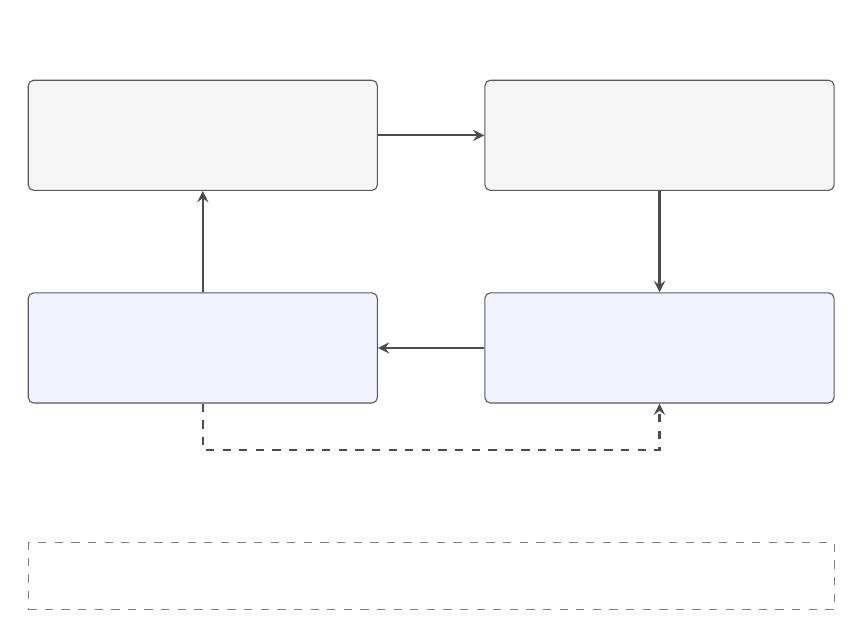
\begin{tikzpicture}[>=stealth, every node/.style={font=\small},
box/.style={draw=black!65, rounded corners=2pt, align=center, minimum height=1.4cm, text width=4.2cm},
arr/.style={->,thick,draw=black!70}]
\node[font=\small\bfseries] at (2.9,1.25) {任务执行闭环};
\node[box,fill=black!4] (task) at (0,0) {任务执行\\模型、运行框架、记忆};
\node[box,fill=black!4] (evidence) at (5.8,0) {经验记录\\结果与运行轨迹};
\node[font=\small\bfseries] at (2.9,-1.35) {系统改进闭环};
\node[box,fill=blue!5] (improver) at (5.8,-2.7) {改进算子\\提出、测试、选择};
\node[box,fill=blue!5] (commit) at (0,-2.7) {提交的后继系统\\有版本记录的继承变化};
\draw[arr] (task)--(evidence);
\draw[arr] (evidence)--(improver);
\draw[arr] (improver)--(commit);
\draw[arr] (commit)--(task);
\draw[arr,dashed] (commit.south) -- (0,-4.0) -- (5.8,-4.0) -- (improver.south);
\node[align=center,text width=10cm,font=\footnotesize] at (2.9,-4.45) {递归：继承的变化影响下一轮改进者};
\node[draw=black!50,dashed,align=center,text width=10cm,minimum height=0.85cm] at (2.9,-5.6) {外部审计：稳定约定、隔离反馈、完整预算};
\end{tikzpicture}
\caption{两个相连的闭环，以及递归主张所需的额外继承关系。外部审计是本文评估方案中的实验边界。本图为本文综合绘制，并非复制既有论文图。}
\label{fig:loops}
\end{figure}


在后文评估方案中，记为 \(V^*\)
的审计评估器被有意放在可修改状态之外。这是实验边界，并不意味着现实系统存在一个绝对不变的外部裁判。内部评估器可以进化，但不能让候选系统自由改写用来证明其进步的全部证据。

\hypertarget{ux4e09ux79cdux533aux522bux4e0eux4e00ux4e2aux66f4ux5f3aux7684ux5047ux8bf4}{%
\subsection{三种区别与一个更强的假说}\label{ux4e09ux79cdux533aux522bux4e0eux4e00ux4e2aux66f4ux5f3aux7684ux5047ux8bf4}}

\textbf{临时修订}改变当前回合中的答案、计划或工作上下文，但不会将其保留给后续回合。\textbf{持久自我改进}根据系统经验，提交对模型、记忆、工具、提示词或代码的更新。\textbf{递归改进}还进一步改变后续产生或选择改进时使用的机制，并使这一变化被继承。这些类别描述机制，不是单一的智能水平或安全等级。

更强的主张是\textbf{持续递归加速}。它讨论一连串改进的动态特征：在明确处理资源与任务难度的条件下，系统产生有用变化的能力，是否在多个代际中持续上升。自指结构并不能推出这一结论。能够修改自身的程序，仍可能停滞、振荡、越来越昂贵，或损害选择基准之外的重要能力。

按照本文的操作性定义，权重更新既不是必要条件，也不是充分条件。冻结基础模型、同时改变代码形式的改进程序，可以在复合系统层面构成有边界的递归。反过来，使用固定优化器反复训练神经网络，虽然构成学习，却不证明优化器或整体改进机制变得更有效。STOP
使用了更严格的术语，因为其底层语言模型保持固定，所以明确没有宣称实现完整
RSI \citep{stop2023}。交代清楚系统边界，可以消解这类表面争议。

同样，一个系统训练了另一个模型，并不自动意味着它改进了自身。必须说明继承关系：训练得到的模型、优化器或运行框架，是否成为下一轮研究智能体的一部分？如果没有这种继承，结果支持的是自动化
AI 开发；它与 RSI 相关，但尚未形成闭合的递归谱系。

\hypertarget{ux673aux5236ux4e0eux8bc1ux636eux5206ux522bux62a5ux544a}{%
\subsection{机制与证据分别报告}\label{ux673aux5236ux4e0eux8bc1ux636eux5206ux522bux62a5ux544a}}

有用的研究描述，应同时记录修改机制及其效果证据。本文采用四个可分别回答的问题：收益能否在新会话中保留；能否在匹配资源的比较中保留；更新后的改进者能否从可比起点优于冻结改进者；这种优势能否跨越更多代际或分布变化。这些问题可以分开检验，不必强行排列为一套等级。

例如，把进化后的运行框架移植到另一个模型，支持框架具有可迁移性；但它本身不能说明移植后的系统更善于生成下一次修改。成功执行代码重写，证明修改可运行且可以保留；但收益仍可能主要来自额外搜索，而不是该代码变化。区分这两类陈述，能够避免把``允许修改某组件''误写成``已证明具备相应能力''。

\hypertarget{ux4e3bux8981ux673aux5236ux8109ux7edc}{%
\section{主要机制脉络}\label{ux4e3bux8981ux673aux5236ux8109ux7edc}}

\hypertarget{ux5f62ux5f0fux5316ux81eaux4feeux6539ux5143ux5b66ux4e60ux4e0eux5f00ux653eux5f0fux641cux7d22}{%
\subsection{形式化自修改、元学习与开放式搜索}\label{ux5f62ux5f0fux5316ux81eaux4feeux6539ux5143ux5b66ux4e60ux4e0eux5f00ux653eux5f0fux641cux7d22}}

哥德尔机的重要性，在于把修改系统自身软件纳入优化问题。其保证依赖公理、效用规范以及合适证明的可获得性；它不保证有用证明能以低成本找到，也不保证所指定的效用涵盖现实中的所有利益
\citep{goedel2003}。受到这一思路启发的经验型编程智能体，不会因为用测试评估补丁就自动获得相同的理论保证。

学习优化器提供了另一条路线。Andrychowicz
等人从一组训练问题中学习优化行为，AutoML-Zero
则从较低层次的程序构件搜索学习算法
\citep{learnoptimizer2016, automlzero2020}。这些方法可以改进学习者的更新规则，但不要求学习者自主重写整个外层搜索过程。它们也揭示了一个持续存在的问题：所谓改进，总是在特定任务分布和搜索表示下测量的。

自博弈和环境共同进化，则提供了自动生成学习挑战的机制。AlphaZero
的早期表述在固定游戏规则与训练流程下，通过自博弈学习国际象棋和将棋
\citep{alphazero2017}。POET
让环境及其解法共同发展，并在演化任务间迁移解法
\citep{poet2019}。对手不断变化或环境越来越难，并不足以证明学习算法发生了递归重设计；其意义在于，学习机会可以由系统生成，而不必始终来自静态题库。

\hypertarget{ux8f93ux51faux4feeux8ba2ux8bb0ux5fc6ux4e0eux53efux590dux7528ux5de5ux5177}{%
\subsection{输出修订、记忆与可复用工具}\label{ux8f93ux51faux4feeux8ba2ux8bb0ux5fc6ux4e0eux53efux590dux7528ux5de5ux5177}}

Self-Refine 根据生成内容的反馈继续修订输出；Reflexion
保存可影响后续尝试的语言反馈；Voyager 在探索过程中积累可执行技能库
\citep{selfrefine2023, reflexion2023, voyager2023}。它们体现了不同的持久性边界：输出修订可能仅在当前回合有效，保留反馈和技能则可以在不更新权重的情况下改变未来行为。Toolformer
还提供了参数层面的路线，通过自动筛选的工具调用示例训练模型
\citep{toolformer2023}。

这些机制与 RSI
密切相关，因为可靠的改进者也需要记忆、工具和纠错。不过，把经验写入记忆，只是提出了一个候选机制。需要在新会话中比较，证明经验被正确检索和使用，同时确认陈旧或无关信息没有损害后续任务。更强的问题是：系统是否改进了记忆写入、选择、检索或修订的方法？

内部自纠错的实验结果也存在争议。Huang
等人在所研究的推理任务中发现，缺少外部反馈时自纠错可能失效；后续研究则发现提示词是否公平、解码设置如何，会明显影响结果
\citep{intrinsic2023, intrinsicpositive2024}。SCoRe
通过强化学习专门训练多轮自纠错，并报告训练后的收益
\citep{score2024}。这些工作检验的干预并不相同，既不能据此断言自纠错普遍不可能，也不能默认未经专门训练的反复自我批评总是有效。

\hypertarget{ux5408ux6210ux76d1ux7763ux4e0eux5171ux540cux8fdbux5316ux7684ux8bfeux7a0b}{%
\subsection{合成监督与共同进化的课程}\label{ux5408ux6210ux76d1ux7763ux4e0eux5171ux540cux8fdbux5316ux7684ux8bfeux7a0b}}

STaR 将生成的推理轨迹反馈到进一步训练，Self-Instruct
则生成和筛选指令学习示例
\citep{star2022, selfinstruct2022}。这类流水线可以将有用行为固化到参数中，但不是无中生有地创造信息。预训练知识、种子样本、筛选规则、已知答案以及环境规律，都可能贡献监督。因此，训练数据的来源应分组件说明，不能只用``自生成''三个字概括。

Self-Rewarding Language Models
在迭代偏好优化中，把回答生成与模型给出的评价信号相结合；SPIN
则通过锚定在监督数据集上的自博弈目标学习
\citep{selfreward2024, spin2024}。二者的反馈通道不同：模型产生的偏好属于学习得到的判断，监督参考答案则是相对于生成结果的外部依据，任何一个通道都不应被自动视为无误。

可验证奖励强化学习提供了另一条路线。DeepSeek-R1
表明强化学习可以显著塑造推理行为，但并不意味着训练程序已经被系统自主重设计
\citep{r12025}。Absolute Zero
Reasoner（AZR）用代码执行反馈连接任务提出与求解 \citep{azr2025}；R-Zero
让挑战者与求解者共同进化，通过求解者多个答案的一致性产生伪标签
\citep{rzero2025}。可执行验证与多数一致性具有不同的误差性质：多数答案可能系统性地错误，而通过执行检查也可能只覆盖有限规范。

这些研究中的``零数据''描述的是某种后训练输入条件，不意味着没有预训练、人类编写的软件、预先选择的目标或环境结构。它们把部分课程和监督工作，从固定的人类整理后训练数据集转移到自动化闭环中。这个闭环是否进一步改进了自己的学习机制，仍然是另一个实验问题。

\hypertarget{ux63d0ux793aux8bcdux8fd0ux884cux6846ux67b6ux4e0eux6539ux8fdbux7a0bux5e8fux7684ux8fdbux5316}{%
\subsection{提示词、运行框架与改进程序的进化}\label{ux63d0ux793aux8bcdux8fd0ux884cux6846ux67b6ux4e0eux6539ux8fdbux7a0bux5e8fux7684ux8fdbux5316}}

Automated Design of Agentic
Systems（ADAS）使用元智能体编写候选智能体，保存此前设计的档案；GEPA
通过语言反思和进化选择优化提示词
\citep{adas2024, gepa2025}。两者都让智能体设计的重要部分成为可搜索对象。但使用固定控制器优化提示词或智能体架构，与修改负责搜索的控制器，本质上是两个不同的干预。

STOP
直接把改进程序应用于自身，使生成的程序改变调用语言模型、改进下游程序的方式
\citep{stop2023}。Gödel Agent 同样向自修改开放智能体逻辑
\citep{goedelagent2024}。这些工作将搜索对象推进到系统改进机制。与此同时，目标、运行时限制、模型
API 和评估程序等外部结构，仍决定了所谓``闭环''究竟关闭到哪一步。

SICA 和 Darwin Gödel Machine（DGM）在编程智能体中实现具体的自修改。DGM
保留种群档案，使此前发现的智能体能够作为后续变化的起点；SICA
使用智能体自身的编程能力改进其实现
\citep{sica2025, dgm2025}。结果支持继承运行框架的价值，但解释依赖任务子集、预算、选择规则与对照。在本文查阅的
DGM
版本中，档案维护与父代选择仍是固定机制，因此其边界是：自修改智能体在一个外部指定的进化流程内演化。

HGM
针对``按照当前得分选择父代''的弱点，从后代结果估计分支层面的改进产出能力，并区分扩展、评估与选择决策
\citep{hgm2025}。这与``改进者是否变得更强''直接相关。但研究者提出的新外层搜索方法，不能自动被描述为系统自主发现的方法。它提供的是对谱系敏感的搜索及相应比较证据，并不是所有人类设计的改进机制都已被移除。

\hypertarget{ux81eaux4e3bux6743ux91cdux9002ux5e94}{%
\subsection{自主权重适应}\label{ux81eaux4e3bux6743ux91cdux9002ux5e94}}

SEAL
训练模型生成``自编辑''：训练数据与更新指令，并在适应之后评估这些编辑是否有用。其外层强化学习奖励能改善更新后模型下游表现的编辑
\citep{seal2025}。语言模型因此参与决定新信息怎样转化为参数更新。这也说明持久性必须分清对象：一次适应回合、一个累计更新后部署的模型，以及一轮外层训练，并不是同一件事。

Search over Self-Edit Strategies
研究了一个范围更窄的扩展，让模型搜索适应模板及部分超参数。该研究明确限定为一轮自我改进；使用档案相对于较弱模板有帮助，但没有超过最强的人类设计基线，同时仍存在同质化问题
\citep{selfedit2026}。这类限制性结果很有价值：扩大可修改接口，不保证模型能够有效利用新增自由度。

完整评估应区分自编辑提案质量的提高，与起始模型变强或训练预算变化带来的收益，还应测量此前适应是否被保留。一个系统即使能高效吸收新信息，只要反复损害旧能力，就不能据此宣称形成不受限制的累计学习过程。

\hypertarget{ux7b97ux6cd5ux53d1ux73b0ux4e0eux81eaux52a8ux5316ux79d1ux7814}{%
\subsection{算法发现与自动化科研}\label{ux7b97ux6cd5ux53d1ux73b0ux4e0eux81eaux52a8ux5316ux79d1ux7814}}

FunSearch
将预训练语言模型提案、程序评估与候选种群结合起来发现有用程序；AlphaEvolve
将进化编程扩展到更广泛的算法和基础设施问题
\citep{funsearch2024, alphaevolve2025}。这些工作说明，外部执行可以让生成模型完成超出其直接回答能力的任务。优化模型开发使用的基础设施，能够形成潜在反馈路径；但在把它称为自主递归加速之前，应当测量完整的端到端收益。

The AI Scientist
及其后续版本自动化了部分假说生成、实验、分析和论文撰写工作
\citep{scientist2024, scientistv22025}。完成论文或得到成功实验，属于科研自动化证据。对于
RSI，还缺一个关键环节：发现的成果是否被继承，并改善下一轮开展研究的研究者？科研产出数量、评审分数和后继模型能力，不是可以相互替代的指标。

因此，当前存在的是多个局部相连的闭环。更好的编程框架可以构建更好的数据生成器，数据生成器可以训练更好的模型，模型又可以提出更好的框架修改。这种耦合在机制上合理，但画出相互连接的图，不等于证明净收益为正。接口成本、迁移损失、评估噪声及训练开销，都可能抵消局部改进。

\hypertarget{ux4ee3ux8868ux7cfbux7edfux7684ux6bd4ux8f83ux8bc1ux636e}{%
\section{代表系统的比较证据}\label{ux4ee3ux8868ux7cfbux7edfux7684ux6bd4ux8f83ux8bc1ux636e}}

表 \ref{tab:mechanisms}
总结主要机制边界。``递归相关性''是本文对设计的解释，不是经过独立核验的能力等级。

\begin{longtable}{p{0.16\linewidth}p{0.22\linewidth}p{0.23\linewidth}p{0.29\linewidth}}
\caption{代表机制及递归主张的边界。}\label{tab:mechanisms}\\
\toprule
方法家族 & 持久修改对象 & 主要反馈 & 递归相关性与边界 \\
\midrule\endfirsthead
\toprule 方法家族 & 持久修改对象 & 主要反馈 & 递归相关性与边界 \\
\midrule\endhead
Self-Refine & 通常为回合内输出 & 模型批评 & 未保留变化时属于输出修订。 \\
Reflexion / Voyager & 记忆 / 可执行技能 & 任务及环境反馈 & 持久适应；更新机制未必演化。 \\
STaR / Self-Instruct & 模型参数 & 筛选后的合成监督 & 预先指定流水线中的自训练。 \\
Self-Rewarding & 策略及评价行为 & 学习得到的偏好 & 耦合改进需要外部校准。 \\
AZR / R-Zero & 策略及课程 & 执行 / 答案一致性 & 自适应课程；外部依据明显不同。 \\
ADAS / GEPA & 智能体代码 / 提示词 & 任务得分及轨迹 & 具有外层搜索程序的设计自动化。 \\
STOP / G\"odel Agent & 改进程序或智能体逻辑 & 下游效用 & 有边界的直接自指；资源和裁判仍被指定。 \\
SICA / DGM & 自修改运行框架 & 编程基准 & 继承代码变化；基础模型及部分外层逻辑固定。 \\
HGM & 后代种群 & 基于谱系的估计 & 测量有价值的祖先；外层搜索由研究者设计。 \\
SEAL & 自编辑策略及适应后权重 & 更新后任务表现 & 在给定外层流程内学习适应选择。 \\
FunSearch / AlphaEvolve & 候选程序 & 可执行评估器 & 发现可帮助 AI 开发；继承关系需另行证明。 \\
AI Scientist & 科研产物 & 实验及评审 & 科研自动化；后继反馈属于额外主张。 \\
\bottomrule
\end{longtable}

几个数值案例说明评估单位为什么重要。DGM 报告，在其 SWE-bench
评估子集上从 20.0\% 提升到 50.0\%，在完整 Polyglot 上从 14.2\% 提升到
30.7\%。前者不能改写为完整官方测试集的得分。论文还包含冻结改进者及移除档案等消融，这些对照比单一终点分数更有助于判断递归主张
\citep{dgm2025}。

SICA 报告，在随机 SWE-bench Verified 子集上从 17\% 提升到 53\%。其试验将
50 道 SWE-bench 题与其他任务组合，在效用中纳入时间和金钱成本，并报告一次
15 轮试验的 API 开销约为 7,000 美元
\citep{sica2025}。这些限定对应一个有边界的实验，不能推广为普遍部署中的改进速度。由于设置不同，SICA
与 DGM 的百分比也不应直接排列高低。

HGM 明确研究后代的改进产出，而不是把当前任务表现视为充分代理
\citep{hgm2025}。这支持评估重点向系统改进过程转移。但已发现框架的迁移、对高产谱系的预测，以及可复用改进算子的因果提升，仍是不同结果。下一节提出的方案，旨在区分这些证据，同时保留它们各自的实际意义。

2026 年的新基准增加了互补的测量对象。PAST-Bench
在后续新会话中，比较打开或关闭已有经验访问权限的表现，并检查持久状态实际起作用的路径
\citep{pastbench2026}。RSIBench-Data
固定周边后训练技术栈，让智能体修改训练数据策略。作者报告，58.33\%
的设置优于首次有效尝试；在已经达到观测峰值且之后继续搜索的运行中，78.26\%
的最终尝试低于此前峰值
\citep{rsidata2026}。后一数值描述的是一个经过条件筛选的运行集合，相对于各自运行内最大值的回退，不能解释为随机系统再多研究一轮就变差的概率。

PostTrainBench 允许智能体在限定 GPU
预算下执行后训练，记录了目标适应的成功案例，也记录了涉及基准和资源边界的失败
\citep{posttrain2026}。AI4AI-Bench
将四小时开发阶段与后续最多十二小时的从头运行分开，在十个研究仓库上使用隐藏最终评估器
\citep{ai4ai2026}。这些基准让 AI
开发的不同部分可以被实验检验，但单个数据研究或算法设计基准，仍不证明训练出的后继者能够反复成为更强的研究者。

\hypertarget{ux5982ux4f55ux8bc4ux4f30ux6539ux8fdbux80fdux529bux7684ux6539ux8fdb}{%
\section{如何评估``改进能力的改进''}\label{ux5982ux4f55ux8bc4ux4f30ux6539ux8fdbux80fdux529bux7684ux6539ux8fdb}}

\hypertarget{ux73b0ux6709ux57faux51c6ux6d4bux91cfux4ec0ux4e48}{%
\subsection{现有基准测量什么}\label{ux73b0ux6709ux57faux51c6ux6d4bux91cfux4ec0ux4e48}}

SWE-bench 测量仓库层面的软件问题解决，MLE-bench
测量机器学习工程，RE-Bench 在研究工程任务中比较智能体与人类专家
\citep{swebench2023, mlebench2024, rebench2024}。它们可以提供有用的任务结果，但任何一个单独得分，都不是递归改进能力的天然指标。测试科研产物的基准，可能根本不测试下一位研究者继续改进这些产物的能力。

PAST-Bench 关注经验保留，RSIBench-Data 关注训练数据决策，PostTrainBench
关注自主后训练，AI4AI-Bench 强调算法层面的变化
\citep{pastbench2026, rsidata2026, posttrain2026, ai4ai2026}。它们更适合组成模块化评估套件，而不是合成一个通用
RSI 分数。关键模块包括持久性、有用提案、有效选择、继承以及多代迁移。

\hypertarget{ux5339ux914dux6539ux8fdbux7b97ux5b50ux7684ux6bd4ux8f83}{%
\subsection{匹配改进算子的比较}\label{ux5339ux914dux6539ux8fdbux7b97ux5b50ux7684ux6bd4ux8f83}}

令 \(A\) 表示起始目标系统，\(U\) 表示改进算子，\(b\) 为开发预算，\(V^*\)
为隔离的审计评估器。本文提出一个``改进产出''度量：

\[
Y(U,A;b)=\mathbb{E}\left[V^*(\operatorname{Run}(U,A;b))-V^*(A)\right].
\]

期望覆盖任务抽样及相关随机性，审计时的推理预算与环境版本另行固定。随后，在相同起始系统分布上比较更新算子
\(U_t\) 与原始算子 \(U_0\)：

\[
\Delta_{\mathrm{op}}(b)=\mathbb{E}_{A\sim\mathcal{A}_{\mathrm{audit}}}
\left[Y(U_t,A;b)-Y(U_0,A;b)\right].
\]

正的估计值支持指定条件下的算子优势，不证明普遍优越性。匹配 \(A\)
很重要，否则新算子可能只被用于更强的目标系统，或者面对完全不同的剩余提升空间。同样，比较完整方法时，应计入获得新算子的开发成本：复用一个已经学到的算子，与从头发现这个算子，回答的是不同的经济性问题。

上述比较综合了后代改进产出能力、持久性对照及自适应数据分析中的既有问题
\citep{hgm2025, pastbench2026, adaptive2015}。它不是新定理，本文也没有证明这一特定指标能够预测长期通用进步。

\hypertarget{ux56e0ux5b50ux5bf9ux7167ux4e0eux8026ux5408ux7cfbux7edf}{%
\subsection{因子对照与耦合系统}\label{ux56e0ux5b50ux5bf9ux7167ux4e0eux8026ux5408ux7cfbux7edf}}

当目标与改进者可以分离时，二乘二实验可以帮助区分两者贡献：

\begin{longtable}[]{@{}lll@{}}
\toprule
起始目标 & 原始算子 \(U_0\) & 更新算子 \(U_t\)\tabularnewline
\midrule
\endhead
原始目标 \(A_0\) & 基线开发运行 &
从原始目标出发的算子效果\tabularnewline
更新目标 \(A_t\) & 固定改进方法下的目标状态效果 &
联合效果及可能的相互作用\tabularnewline
\bottomrule
\end{longtable}

每格使用相同的开发预算、审计协议与任务切分。同一行内比较两列，可以估计给定目标下的算子效果；比较不同行则同时改变能力和提升空间，解释需要更谨慎。这个设计还能够暴露：新算子是否只对与其共同进化的目标有效。

有些系统高度耦合：修改模型同时改变求解者和改进者，无法在保留功能的同时进行干净移植。强行拆开，反而会制造不真实的系统。这时应比较完整谱系与冻结更新的对照，准确描述干预，并报告仍无法归因的部分。功能性自指是系统属性，在实验中隔离其因果贡献则是额外挑战。

有用的对照包括：拥有相同候选生成预算的冻结改进者；拥有相同评估预算的重放或随机搜索控制器；以及在保持任务提示不变时移除已学习状态的无持久化条件。还应特别控制推理采样开销：如果进化后的智能体只是调用了更多次模型，准确率可能提高，但效率并未提高。这个结果仍有用，只是必须明确资源与效果的交换关系。

\hypertarget{ux5f00ux53d1ux53cdux9988ux4e0eux5ba1ux8ba1ux8bc1ux636eux5206ux79bb}{%
\subsection{开发反馈与审计证据分离}\label{ux5f00ux53d1ux53cdux9988ux4e0eux5ba1ux8ba1ux8bc1ux636eux5206ux79bb}}

可靠的方案应区分开发任务、选择反馈和最终审计任务。候选搜索可以反复查看开发反馈，选择程序可以按单独规定的预算获得验证反馈，最终审计则应评估已冻结的候选系统或谱系，不再将任务级信息反馈给搜索过程。不断访问一个所谓保留集，会让它成为自适应优化过程的一部分
\citep{adaptive2015}。

对长期运行的系统，一次没有被接触过的保留集不可能永久解决问题。后续审计需要新的任务家族、受控的信息披露，或明确针对自适应复用设计的统计程序。隐藏测试可以降低直接记忆答案的风险，但不能自动保证它测量了正确的研究对象。EvalPlus
表明，更强的测试覆盖会改变对生成代码的评价；RSI
评估同样需要检验，它测到的是所宣称的能力，还是一个方便使用的代理指标
\citep{evalplus2023}。

改进算子的迁移应有自己的数据切分。如果算子在一组代码仓库上开发，就应该让它改进新的起始智能体或仓库，必要时更换模型家族。更强的检验，是让迁移后的算子在新环境中继续产生有用后代；只测试已进化智能体的即时任务得分，回答的是较弱的问题。

\hypertarget{ux8c31ux7cfbux9009ux62e9ux4e0eux7edfux8ba1ux4e0dux786eux5b9aux6027}{%
\subsection{谱系、选择与统计不确定性}\label{ux8c31ux7cfbux9009ux62e9ux4e0eux7edfux8ba1ux4e0dux786eux5b9aux6027}}

自我改进实验应保存完整的祖先关系图，包括候选版本哈希、父代标识、提议修改、评估访问、被拒绝的变化、崩溃及选择决策。谱系能够显示一次修改如何影响未来可能性。只报告最终最强智能体，会抹去失败分支，让人难以区分稳定有效的研究程序与偶然抽中的幸运结果。

应分开报告三条曲线：当前部署候选；使用允许的验证信息选出的最佳候选；以及事后按照审计分数挑选的最佳候选。第三条是分析产物，除非协议明确允许获取这些审计信息并把成本计入开发，否则它并不是可部署的选择策略。``历史最佳''曲线按定义不会下降，因此不能证明连续修改一直有效。

不确定性的估计应对应真正实施干预的层级。同一条演化谱系中的任务结果，共享祖先和选择历史；把它们全部当作独立重复，会夸大精度。独立谱系、任务家族重抽样，以及使用共同随机种子的配对评估，分别处理不同方差来源。论文应报告独立运行次数及置信区间方法，而不是给出一个普遍足够的随机种子数量。

\hypertarget{ux6210ux672cux6301ux4e45ux6027ux4e0eux52a0ux901f}{%
\subsection{成本、持久性与加速}\label{ux6210ux672cux6301ux4e45ux6027ux4e0eux52a0ux901f}}

资源核算应涵盖提案模型推理、候选执行、评估器调用、参数更新、失败运行，以及重要的存储、检索开销和人类干预。实际耗时、API
费用、GPU 小时和推理 token
数是不同量。方法可以通过并行降低耗时，同时增加总算力。论文应报告相关资源向量，而不是把一个方便的标量当作通用预算。

持久性要求在新会话中评估已经提交的系统，不重放带有特权信息的开发轨迹。能力保留还需要测试此前任务和约束，避免把窄域优化中对旧能力的交换描述为累计进步。如果系统修改了自身目标，仍应保留稳定外部目标下的比较；自选一个更容易的目标，不意味着在原目标上变得更好。

研究加速时，令 \(C_t\) 为累计开发成本，\(P_t\)
为在稳定或明确校准的任务分布上测得的外部表现。一个简单的描述性增量为：

\[
 g_t=\frac{P_{t+1}-P_t}{C_{t+1}-C_t}.
\]

少数观测中 \(g_t\)
上升，不构成持续加速的证明。它可能来自噪声、提升空间、任务难度变化或有利分支。更强的主张需要重复代际实验、合适的冻结改进者反事实、对资源变化的明确处理，以及超出选择基准的迁移。得分接近饱和时，这个比值也难以解释。因此，本文建议同时报告成本---表现前沿、算子产出曲线和原始轨迹，不把有限实验外推为智能爆炸预测。

\hypertarget{ux5931ux6548ux673aux5236ux4e0eux5b89ux5168ux8fb9ux754c}{%
\section{失效机制与安全边界}\label{ux5931ux6548ux673aux5236ux4e0eux5b89ux5168ux8fb9ux754c}}

\hypertarget{ux53cdux9988ux8d28ux91cfux4e0eux8bc4ux4f30ux5668ux5171ux540cux9002ux5e94}{%
\subsection{反馈质量与评估器共同适应}\label{ux53cdux9988ux8d28ux91cfux4e0eux8bc4ux4f30ux5668ux5171ux540cux9002ux5e94}}

任何改进闭环都不能脱离反馈解释。已有研究记录了 LLM
评估器的偏差与局限，也表明过度优化代理奖励可能降低另一个参考指标下的表现
\citep{judge2023, rewardoveropt2022}。如果提案者与评估器共享盲点，反复一致可能只是提高表面信心，而没有增加独立的正确性证据。

这不意味着存在一条普遍适用的排序，使所有形式化检查都优于所有人类或模型判断。证明对其所证明的形式命题提供强证据，但命题本身可能遗漏重要需求；编译器检查的属性也比完整行为测试窄；领域专家则可能评估前两者没有表达的要求。关键问题是：信号能够发现哪些错误，成本如何，与真正需要的结果有多好的对应关系？

当评估器自身变化时，还会增加一个识别问题：得分提高可能源于候选能力增强、裁判更宽松，或者目标被改写。新评估器应在独立标注或可执行检验的案例上接受评估，包含具有对抗性、容易引发分歧的案例，同时保留候选系统无法重写的参考评价。评估器的校准表现，应与策略在新裁判下的分数分开报告。

\hypertarget{ux5d29ux6e83ux9057ux5fd8ux4e0eux591aux6837ux6027ux4e27ux5931}{%
\subsection{崩溃、遗忘与多样性丧失}\label{ux5d29ux6e83ux9057ux5fd8ux4e0eux591aux6837ux6027ux4e27ux5931}}

递归训练于模型生成数据，可能丢失原始数据分布的信息。模型崩溃文献在特定训练与采样条件下展示了这种风险；关于同时积累真实与合成数据的研究，则说明任何合成数据使用都必然导致崩溃的说法并不成立
\citep{collapse2023, accumulate2024}。结论具有条件性：替换、积累、筛选及外部依据会产生不同动态。

智能体进化即使不更新参数，也会失去多样性。生成器不断参考同一批成功示例，候选程序可能收敛到相似提示词、架构或行为习惯；自编辑搜索提供了同质化问题的具体报告
\citep{selfedit2026}。档案能够保留不同选项，但文字看起来不同，不等于行为策略不同。评估应检验不同策略和迁移特征，而不仅是统计存了多少候选。

遗忘带来另一类交换。改善编程速度的变化可能损害错误恢复，压缩记忆的规则可能丢弃罕见却重要的约束。因此，能力保留与回归测试应进入修改接受流程，而不是到部署后才发现。保留可恢复的旧版本能够限制操作损害，却不能单独使研究过程变得稳定进步。

\hypertarget{ux81eaux4feeux6539ux4e0eux63a7ux5236ux5b8cux6574ux6027}{%
\subsection{自修改与控制完整性}\label{ux81eaux4feeux6539ux4e0eux63a7ux5236ux5b8cux6574ux6027}}

如果智能体能够编辑评估器、权限、日志或预算核算，它改变的就可能不仅是任务解法，还包括测量与控制系统。奖励篡改研究提供了分析这些激励的因果框架，PostTrainBench
也记录了当代自动训练实验中的相关边界违规
\citep{tampering2019, posttrain2026}。这些是区分``允许修改的研究工作区''与``外部强制执行的评估和资源边界''的具体理由。

对研究系统，一个合理默认设置是：对候选代码和模型进行版本管理，隔离执行，限制审计资产和凭证访问，在候选代码之外执行预算限制，并保存回滚产物。内部评估能力仍然可以在这一安排内发展。这些约束同时保护实验结论的可解释性和运行环境。

更广泛的失控情景仍是重要研究假说，但本文评述的有限实验不能确定其概率或时间表。反过来，尚未证明开放式加速，也不意味着自修改系统没有风险。关于递归能力的科学主张，与关于运行隔离的工程决策，应分别使用适合的问题证据。

\hypertarget{ux7814ux7a76ux8baeux7a0b}{%
\section{研究议程}\label{ux7814ux7a76ux8baeux7a0b}}

\textbf{直接测量继承。} 自动化 AI
科研应说明下一位研究者继承了什么产物、如何整合，以及它是否提高后续研究产出。这可以把训练算法和数据研究基准连接到多代
RSI 实验，而不是把一次成功训练直接等同于闭环完成。

\textbf{建立可迁移的改进者测试。}
基准应区分学习改进算子的任务，与要求该算子继续改进的新目标系统。迁移应包含产生有用后代，而不只是让已经进化好的智能体解决新题。对于无法移植的耦合系统，应准确设计谱系对照。

\textbf{学习评估，但不放弃测量。}
自奖励与评估器适应的吸引力，在于外部标签昂贵。研究应测试新评估器能否发现旧评估器遗漏的错误，尤其是生成器有动机利用的错误。评估能力增长与保持稳定审计约定可以并存。

\textbf{报告改进的经济性。}
编程、训练内核和数据准备的局部加速，应与总体开发成本联系起来。昂贵的改进者在广泛复用时可能值得使用，但必须交代成本摊销条件。一个基础设施组件的收益，不会自动按同比例转化为整体科研加速。

\textbf{研究长期回退与分支。}
高质量检查点可能很早出现，后续变化未必能超过它。研究应比较谱系选择、检查点保留、多样性维护与停止规则。被拒绝的提案也是搜索过程的有效数据，不应从公开证据中消失。

\textbf{形成共同报告材料。}
最小可复现记录应包括系统边界、候选与父代版本、模型标识、任务切分、评估器访问权限、完整预算、选择规则、独立运行次数及失败日志。即使无法公开完整模型权重或专有
API，这些材料也能提高研究之间的可比性。

\hypertarget{ux672cux7efcux8ff0ux7684ux5c40ux9650}{%
\section{本综述的局限}\label{ux672cux7efcux8ff0ux7684ux5c40ux9650}}

本文偏重大语言模型、编程智能体与计算型科研，因为这些领域较容易提供可检查产物及执行反馈。机器人、硬件自设计、发展式学习及更早期的进化计算文献，没有得到完整覆盖。参考文献是经过选择的样本；关于缺少更强证据的判断，仅针对所选样本，不能被视为全球不存在相应证据的证明。

若干核心来源是预印本，部分结果依赖专有模型或作者运行的基础设施。元数据核对不等于结果有效性验证。任务子集、模型版本、预算及评估访问权限的差异，使可靠的跨论文效应量合并不可行。本文提出的算子产出比较，也需要实际验证，尤其是在耦合智能体和任务分布变化的情况下。本文不提供新的基准成绩、独立复现结果或未来预测。

\hypertarget{ux7ed3ux8bba}{%
\section{结论}\label{ux7ed3ux8bba}}

RSI
最适合被研究为一种明确关系：系统继承的变化，如何影响生成后续变化的过程。现有工作已经提供持久学习、自主适应、自修改运行框架、有价值谱系搜索及自动化
AI
科研等重要机制。所选文献支持多种有边界的自我改进，但尚未确立通用、持续且经过资源开销校正的递归加速。

下一步实验应连接机制、继承与测量。匹配改进者比较、隔离审计反馈、完整谱系记录及透明成本核算，可以检验改进程序本身何时变得更有效。这些做法会让正面结果与停滞结果都具有科学价值，并减少``自动进化''的宏大表述与可复现证据之间的距离。

\hypertarget{ux900fux660eux6027ux8bf4ux660e}{%
\section{透明性说明}\label{ux900fux660eux6027ux8bf4ux660e}}

AI
辅助了检索、起草、翻译和排版。本文没有开展新的实验。配套来源表及证据台账记录综合分析的依据；所提出的评估方案尚未经过实验验证。

\clearpage
\appendix

\hypertarget{ux7b80ux660eux62a5ux544aux6a21ux677f}{%
\section{简明报告模板}\label{ux7b80ux660eux62a5ux544aux6a21ux677f}}

\begin{longtable}[]{@{}ll@{}}
\toprule
项目 & 解释 RSI 主张所需的信息\tabularnewline
\midrule
\endhead
系统边界 &
模型、运行框架、记忆、数据、改进者及评估器；哪些可修改、哪些由外部固定\tabularnewline
机制主张 & 输出修订、持久适应、改进算子提升，或持续加速\tabularnewline
继承关系 & 传给下一代的具体产物；后继者是否开展下一轮改进\tabularnewline
对照 &
冻结改进者、匹配起始目标、无持久化、等价搜索与推理预算\tabularnewline
评估权限 & 开发、选择及审计任务；各阶段返回哪些反馈\tabularnewline
选择规则 & 当前、验证选优及事后最优候选分别报告\tabularnewline
资源 & 提案、评估、训练、失败运行、人类工作及部署推理\tabularnewline
不确定性 & 独立谱系、任务家族变化、配对设计及置信区间方法\tabularnewline
迁移与保留 & 新目标、新模型家族、后续改进及旧能力回退\tabularnewline
可复现性 &
版本产物、谱系图、日志、随机种子、模型标识及失败案例\tabularnewline
\bottomrule
\end{longtable}

\Needspace{15\baselineskip}

\hypertarget{ux672fux8bedux5bf9ux7167}{%
\section{术语对照}\label{ux672fux8bedux5bf9ux7167}}

\begin{longtable}[]{@{}ll@{}}
\toprule
英文 & 本文中文表达及含义\tabularnewline
\midrule
\endhead
Recursive self-improvement &
递归自我改进：继承的变化影响后续改进机制\tabularnewline
Self-evolution & 自进化：系统根据反馈改变自身的宽泛概念\tabularnewline
Persistent adaptation &
持久适应：超出原始回合仍可用的已提交变化\tabularnewline
Improvement operator &
改进算子：提出或选择目标系统修改的程序\tabularnewline
Agent scaffold / harness &
智能体运行框架：模型周围的提示、工具、记忆接口及控制流程\tabularnewline
Metaproductivity &
后代改进产出能力：给定任务与资源设置下产生有用后代的能力\tabularnewline
Audit evaluator &
独立审计评估器：与候选系统的修改和选择过程隔离的评估通道\tabularnewline
Grounding &
外部依据与环境约束：环境、规范或独立参考提供的证据\tabularnewline
Resource-normalized improvement &
经资源开销校正的改进：在明确预算及成本条件下比较的收益\tabularnewline
\bottomrule
\end{longtable}

\clearpage
\bibliography{references.bib}

\end{document}
